\chapter{State of the art} % Main chapter title
\label{StateOfTheArt}

\section{Volume rendering algorithms}

The fundamental volume visualization algorithms described
below fall into two main categories: 

\begin{itemize}

\item Direct volume rendering (DVR) algorithms: they include approaches such as ray-casting, texture mapping, splatting, and V-buffer rendering. Splatting and V-buffer are also called projection methods. These these methods are characterized by mapping elements directly into screen space without using geometric primitives as an intermediate representation.

\item Surface-fitting (SF) algorithms : they are also called isosurfacing or feature-extraction. These algorithms consist in fitting surface primitives such as
polygons or patches to constant-value contour surfaces in volumetric datasets. The surface primitives used are most of the time planar.

\end{itemize}

DVR methods are especially appropriate for creating images from datasets containing amorphous features like clouds, fluids, and gases. One disadvantage of using DVR methods
is that the entire dataset must be traversed each time an image is
rendered. A low resolution pass or random sampling of the data is
sometimes used to create low-quality images quickly for parameter
checking. The process of successively increasing the resolution
and quality of a DVR image over time is called progressive
refinement.

 The user begins by choosing a threshold value
and then geometric primitives are automatically fit to the high-contrast
contours in the volume that match the threshold. Cells
whose comer-values are all above the chosen threshold (cell is
inside) or all below the threshold (cell is outside) are discarded and
have no effect on the final image. Showing just the cells falling on
the threshold is sometimes useful, but can be a problem. Another
consideration is the huge number of surface primitives generated
for large volumetric datasets. 


Many steps in the volume visualization process are common to
volume visualization algorithms.  Most of the fundamental volume
visualization algorithms include only a subset of the steps listed
here.
The initial step in every procedure is data acquisition. The next
common step is to pat the data slices into a form that can be worked
with and then to process each slice so that it covers a good
distribution of values, is high in contrast, and is free of noise and
out-of-range values. Of course, the same set of processes must be
applied to every slice.
Next, the dataset is reconstructed so that the ratio of the
dimensions is proportional to the ratio of the dimensions of the
measured substance or substance being simulated. This may
involve interpolating between values in adjacent slices to construct
new slices, replicating existing slices, interpolating to estimate
missing values, or scan-converting an irregular grid or non-orthogonal
grid onto a Cartesian grid by interpolation. At this point
three-dimensional enhancement may be applied, such as a slight
blurring of the data values. Next, a data-classification or
thresholding is performed. This step will be discussed in detail in
the section on data classification.
After data-classification, a mapping operation is applied to map
the elements into geometric or display primitives. This is the stage
that varies the most between algorithms, as will be shown in the
section on volume visualization algorithms. At this point the
primitives can be stored, manipulated, intermixed with externally
defined primitives, shaded, transformed to screen space, and
displayed. The shading and transformation steps can be reordered
and shading can be done in one of eleven ways as explained in 


\subsection{Direct Volume Rendering}

\subsubsection{Texture mapping}

\paragraph{2D Texture mapping}
2D Texture mapping consists in representing the whole volume as a set of slices parallel to coordinate planes. To create images of the slices, one can use the standard texture mapping capabilities provided by graphics libraries like OpenGL. \ref{fig:2dslices} shows how pixel colors and opacities are calculated when rendering a texture-mapped polygon. In texture mapping, texture coordinates (s, t) are stored along with each vertex. These coordinates are interpolated across the polygon during scan conversion, and are used as coordinates for color look-up inside a texture image \ref{fig:2dtexture}. Color and opacity values from the texture image are reconstructed using bi-linear interpolation.


\begin{figure}[th]
\centering
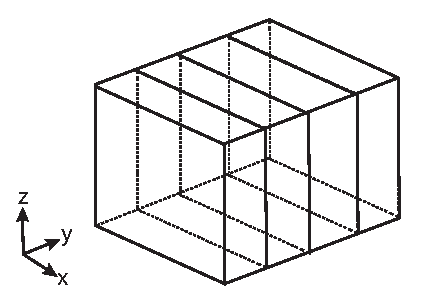
\includegraphics{Figures/2D_slices}
\decoRule
\caption[2D Sclices]{2D slices of the volume.}
\label{fig:2dslices}
\end{figure}
On modern graphics workstations, the complete process of interpolating texture coordinates and reconstructing texture values is incorporated into the scan-conversion process and done completely in hardware. Because texture mapping is such a common application, these routines are well-optimized and highly efficient.
To simulate ray casting using texture mapping, we have to slice the volumetric data set into parallel slices, and the use these slices as texture images to texture-map the projections of the sliced onto the image plane. To composite the slices, we can use the blending operations provided by the OpenGL graphics library. As it happens, one of the standard operators provided is exactly the compositing operator used in ray casting. Since compositing is also fully hardware-assisted, it is also very fast.
\begin{figure}[th]
\centering
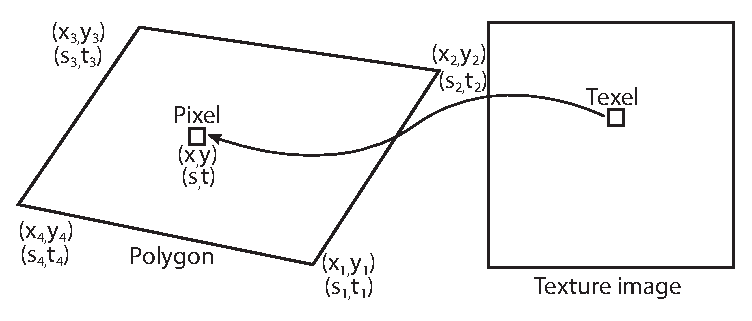
\includegraphics{Figures/2dtexmapping}
\decoRule
\caption[2D texture mapping]{Calculating color and opacity of a pixel inside a texture-mapped polygon.}
\label{fig:2dtexture}
\end{figure}

There are two ways to deal with varying viewpoints.

The first one is to create slice images for the given data set in a pre-processing step and uses different projection matrices to create arbitrary-viewpoint images of these slices. This is fast, since the (expensive) step of slice creation has to be done only once. On the other hand, image quality suffers because the views of all slices will be distorted due to the projection onto the image plane. In the extreme case of the view direction being parallel to the slices, there will be no image at all.

The second way is to create slices which are always orthogonal to the viewing direction. This results in optimal image quality, but it means that the slice stack has to be re-generated for each new image. Furthermore, arbitrary ("oblique") slices through a cuboid are generally not square or rectangular, and can be anything from triangles to hexagons.

\begin{algorithm} \caption{Volume Rendering using 2D Texture Mapping Algorithm} 
\label{alg:tex2dmapping}
\begin{algorithmic}[1]
\Require $N$ the number of slices, $\vec{v} $ the view direction
\State Load the data $\mathcal V(x,y,z) \gets data$ 
\State create the slices $s_i \in \mathcal V$ with each normal $\vec{n_i} \parallel \vec{v}$
\State Turn off the Depth test 
\State Enable the Blending 

\ForEach {$s_i \in \mathcal V $ form back to front}
\State $Texture \gets s_i$
\State create a polygon $p$ corresponding to the slice $s_i$
\State Assign texture coordinates to four corners of the polygon
\State Render and blend the polygon (alpha blending) 
\EndFor

\end{algorithmic}
\end{algorithm}

\paragraph{3D Texture mapping}
To allow interactive generation of view-orthogonal slices, a special hardware technique has been developed. This is a generalization of texture-mapping to three-dimensional textures, appropriately called "3D texturing."
As seen in Figure \ref{fig:2dtexture}, 2D texture-mapping interpolates two additional coordinates (s, t) across a polygon's interior. In 3D texture-mapping, three additional coordinates (s, t, r) are interpolated. To determine a pixel's color and opacity, these three coordinates are used as indices into a three-dimensional image, the 3D texture, see Figure \ref{fig:3dtexture}. To reconstruct texture values, tri-linear interpolation is used.

3D textures allow direct treatment of volumetric data. Instead of generating a set of two-dimensional slices in a pre-processing step, the volumetric data is directly downloaded into the graphics hardware, and is directly used to calculate color and opacity values for each pixel covered by a rendered primitive.

\begin{figure}[th]
\centering
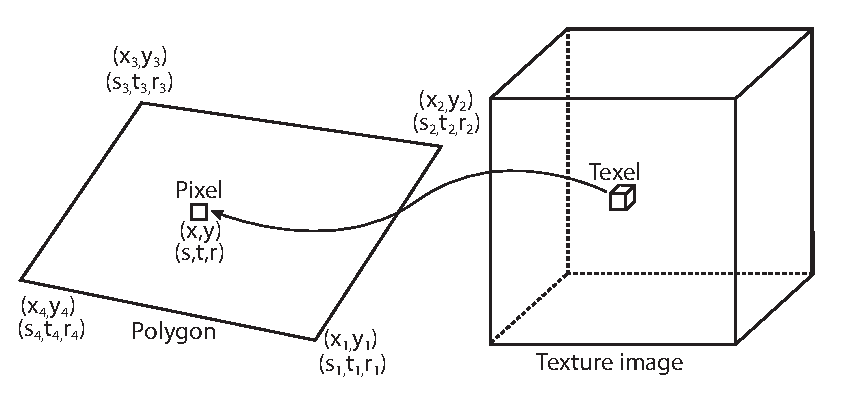
\includegraphics{Figures/3dtexmapping}
\decoRule
\caption[3D texture mapping]{Calculating color and opacity of a pixel inside a texture-mapped polygon using 3D texture.}
\label{fig:3dtexture}
\end{figure}


To generate oblique slices using 3D texturing, one only has to calculate the vertices of the slice, and then to generate the correct 3D texture coordinates for those vertices, see Figure \ref{fig:cubeSlice}. Then these coordinates are passed to the graphics library, and the graphics library will render the projection of the slice onto the image plane, using tri-linear interpolation to reconstruct each pixel's color and opacity values.

\begin{figure}[th]
\centering
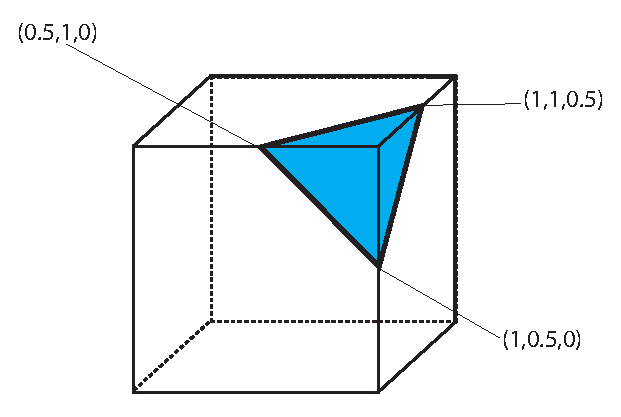
\includegraphics{Figures/cubeSlice}
\decoRule
\caption[3D Cube slice]{Calculating vertex coordinates and texture coordinates for an oblique slice. In this figure, the vertex and texture coordinates are identical.}
\label{fig:cubeSlice}
\end{figure}

\subsubsection{Raycasting}
Volume raycasting computes a 2D image from the 3D volumetric data set.The basic goal of ray casting is to allow the best use of the three-dimensional data and not attempt to impose any geometric structure on it. It solves one of the most important limitations of surface extraction techniques, namely the way in which they display a projection of a thin shell in the acquisition space. Surface extraction techniques fail to take into account that, particularly in medical imaging, data may originate from fluid and other materials which may be partially transparent and should be modeled as such. Ray casting doesn't suffer from this limitation. This algorithm can be split in four main steps (see Figure \ref{fig:rayasting}) :
\begin{itemize}

\item \textbf{Ray casting}. For each pixel of the final image, a ray of sight is shot ("cast") through the volume. At this stage it is useful to consider the volume being touched and enclosed within a bounding primitive, a simple geometric object (usually a cuboid) that is used to intersect the ray of sight and the volume.

\item \textbf{Sampling}. Along the part of the ray of sight that lies within the volume, equidistant sampling points or samples are selected. In general, the volume is not aligned with the ray of sight, and sampling points will usually be located in between voxels. Because of that, it is necessary to interpolate the values of the samples from its surrounding voxels (commonly using trilinear interpolation).

\item \textbf{Shading}. For each sampling point, a transfer function retrieves an RGBA material colour and a gradient of illumination values is computed. The gradient represents the orientation of local surfaces within the volume. The samples are then shaded (i.e. coloured and lit) according to their surface orientation and the location of the light source in the scene.

\item \textbf{Compositing}. After all sampling points have been shaded, they are composited along the ray of sight, resulting in the final colour value for the pixel that is currently being processed. The composition is derived directly from the rendering equation and is similar to blending acetate sheets on an overhead projector. It may work back-to-front, i.e. computation starts with the sample farthest from the viewer and ends with the one nearest to the viewer. This work flow direction ensures that masked parts of the volume do not affect the resulting pixel. The front-to-back order could be more computationally efficient since, the residual ray energy is getting down while ray travels away from camera; so, the contribution to the rendering integral is diminishing therefore more aggressive speed/quality compromise may be applied (increasing of distances between samples along ray is one of such speed/quality trade-offs).

\end{itemize}

\begin{figure}[th]
\centering
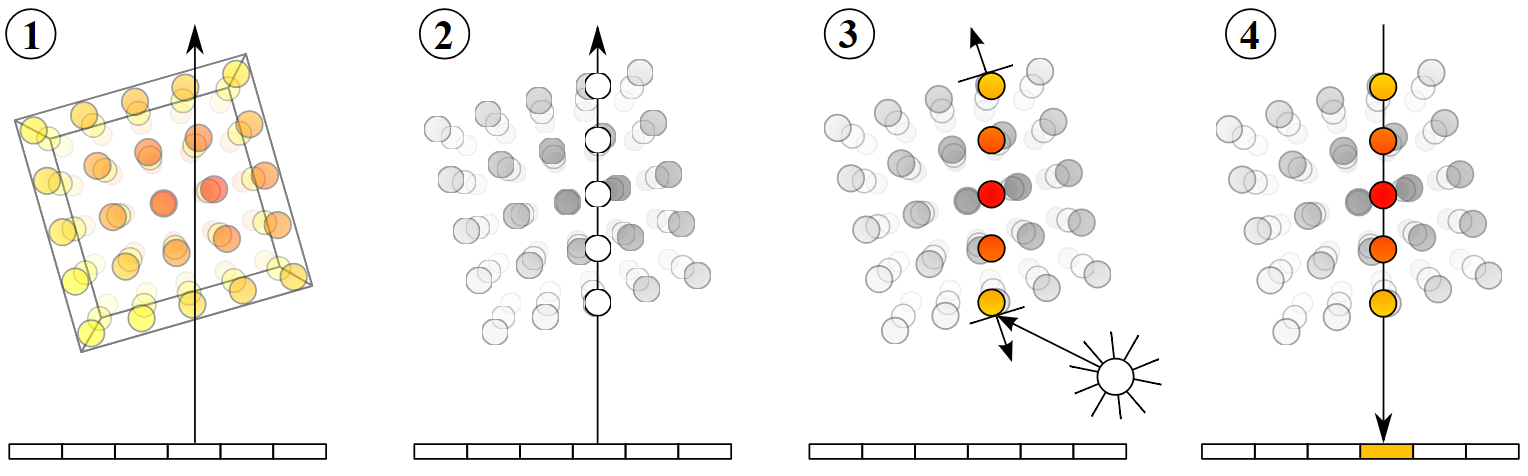
\includegraphics[width=\textwidth]{Figures/raycasting}
\decoRule
\caption[Volume raycasting]{ The four steps of the volume raycasting algorithm  }
\label{fig:rayasting}
\end{figure}

\subsection{Surface-fitting}


\section{Occlusion management strategies}



\subsection{Transfer Function}

A transfer function (TF) maps volumetric data to optical properties
and is part of the traditional visualization pipeline: data acquisition,
processing, visual mapping, and rendering. Volumetric data is
considered to be a scalar function from a three-dimensional spatial
domain with a one-dimensional range (e.g., density, flow magnitude,
etc.). Image generation involves mapping data samples through the
TF, where they are given optical properties such as color and opacity,
and compositing them into the image.
A TF simultaneously defines which parts of the data are essential
to depict and  how to depict these, often small, portions
of the volumetric data. Considering the first step, a TF is a special,
but important, case of a segmentation or classification. With classifi-
cation, certain regions in a three-dimensional domain are identified
to belong to the same material, such as bone, vessel, or soft tissue,
in medical imaging. A plethora of classification and segmentation
algorithms have been developed over the last decades, with semiautomatic
approaches often tailored to specific application scenarios.
Segmentation algorithms can be quite intricate since information
from the three-dimensional spatial domain and the one-dimensional
data range are taken into account. TFs in their basic form are, on the
other hand, restricted to using only the data ranges. In comparison
with general classification algorithms, this characteristic makes a
TF less powerful with respect to identifying relevant parts of the
data. The advantage of a TF is, however, a substantial performance
gain as classification based on the one-dimensional data range reduces
the complexity tremendously. This gain is the result of the
three-dimensional domain being typically two orders of magnitude
larger than the small data range. Histograms are an example of discarding
potentially complex spatial information and aggregating
only the data values to binned-frequency information. In the same
spirit, TFs classify interesting parts of the data by considering data
values alone. The second functionality of a TF deals with specifying
optical properties for portions of the data range previously identified
as being relevant

The transfer functions can be classified according to different criteria. Some of the most important are:

\begin{itemize}
\item \textbf{The dimension: } The one-dimensional TF classifies the scalar data value, $d$, and subsequently maps the material to an optical property for rendering: $ \textbf{q}(d)=\textbf{V}(\textbf{M}(d))$ where $\textbf{M}(.)$ is the material classification function and $\textbf{V}(.)$ is the
visual mapping of the material. One-dimensional TFs are adequate in many cases of simulation data where measurement noise is low or even non-existent where different materials of interest have few overlapping intensity
ranges \cite{4303986}. One-dimensional TFs are often the first tool available in software packages providing volume rendering, as they are relatively easy to comprehend for the novice or occasional user. Practically all production
visualization software, such as ParaView by \cite{paraview},
 VisIt by \cite{Childs:SciDAC2011}, 
or ImageVis3D by {\cite{Fogal2010Tuvok}}, support 1D TF editors.

\begin{figure}[th]
\centering
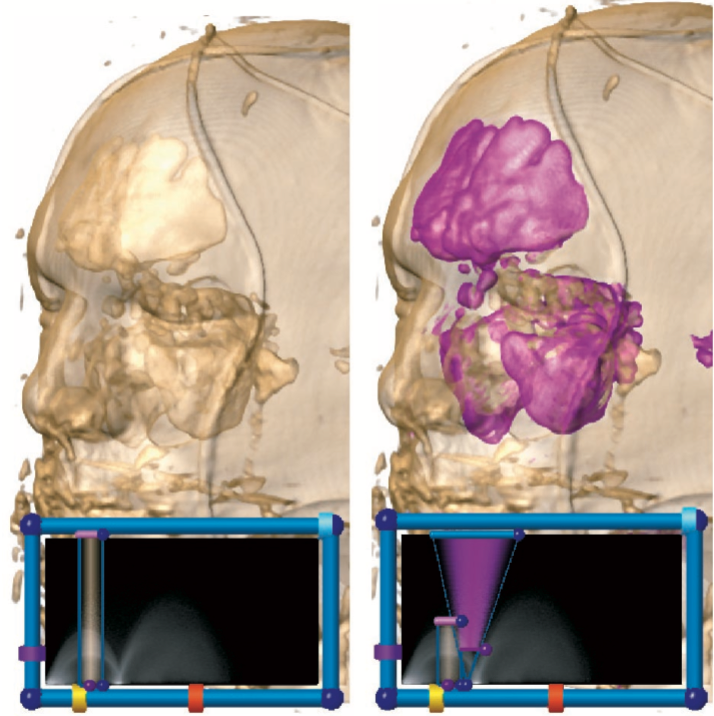
\includegraphics[width=\textwidth]{Figures/2dtf}
\decoRule
\caption[2D transfer Function]{ The two-dimensional TF editor widgets allow the user
to more precisely control the classification power of the 2D TF.
The triangular widget can also be skewed to better fit the desired
classification domain (\cite{1021579}) }
\label{fig:tf2d}
\end{figure}

Multidimensional TFs are used for Multidimensional data. If the user has to manipulate the TF definition directly, moving beyond
2D TFs immediately poses significant challenges in terms of
user interfaces and cognitive comprehension (\cite{1021579}). Much research and
work on Multidimensional TFs is, therefore, related to various forms of automation
and advanced user interfaces. Typical approaches include dimensional reduction, clustering
and grouping, machine learning, and various user interface
approaches such as parallel coordinates by \cite{5742368} or direct slice or volume
view interaction. 

\begin{figure}[th]
\centering
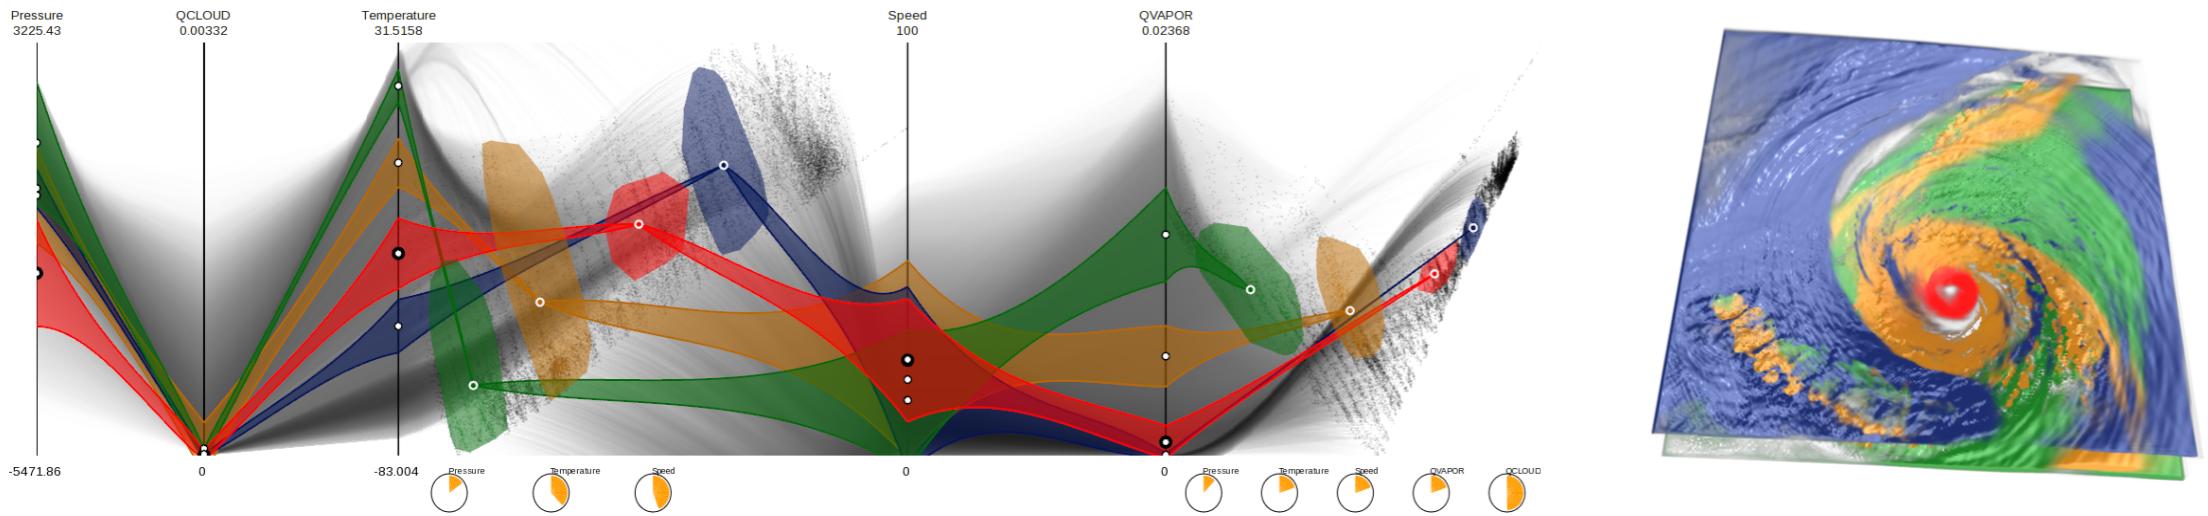
\includegraphics[width=\textwidth]{Figures/mdtf}
\decoRule
\caption[Multidimensional transfer Function]{ Parallel coordinates with embedded multidimensional scale plots for editing multidimensional TFs(\cite{5742368}) }
\label{fig:tfmd}
\end{figure}


\item \textbf{The automation}: The automation includes techniques such as adapting presets, semi-automatic, automatic, and supervised machine learning. Volume rendering has established itself as
a powerful visualization tool in many domains, but the necessary
design of TFs is a time consuming and tedious task. Consequently,
a significant amount of work is dedicated to the automatic and semiautomatic generation of TFs. 

\item \textbf{The aggregated attributes} : Conceptually, the introduction of additional quantities in the TF definition makes it possible to discriminate more parts in a dataset. Histogram clustering helps to reduce the degrees of freedom in designing a TF. As an illustration, \cite{5887324} propose modeling the
histogram space using a Gaussian mixture model. An elliptical TF
is assigned to each Gaussian, and the user interaction is simplified in order to edit the parameters of these ellipsoids.  

\end{itemize}

\subsection{Segmentation}

\subsection{Deformations and Focus + Context}

%%camera !!!!!!!!!!!!!!!!!!!!!!!!!!!!!!!!!!!
\cite{5613463} Almost all images used in visualization are computed with a planar pinhole camera (PPC). One reason for this is that the PPC models the
human eye well, producing images that resemble what users would
see if they were actually looking at the dataset to be visualized.
Another reason is simplicity: software and hardware
implementations of PPC rendering algorithms allow visualizing
complex 3-D datasets at interactive rates. However, the simplicity of
the PPC model also brings three important limitations. First, the PPC
has a limited field of view. Second, the sampling rate of the PPC is
uniform over its entire field of view. Third, the PPC has only a single
viewpoint, i.e. the pinhole where all rays converge. 

An interactive lens is a lightweight tool to solve a localized visualization problems by temporarily altering a selected part of the visual representation of the data~\cite{CGF:CGF12871}. Using this lens approach, we propose an interactive volume deformation based on GPU accelerated ray-casting to free a designated target from local occlusion while keeping the global context.

A lens is a parameterizable selection according to which a base visualization is altered. Typically, a lens is added to a visualization to interactively solve a specific localized problem. This property is very interesting with the aim of providing a focus+context solution to occlusion in volume rendering. Lenses can have different geometric properties not only defining their appearance, but also determining the selection, which is the subset of the data where these lenses take effect. The major geometric properties of a lens are shape, position, and size as well as the orientation.
The shape of a lens is usually chosen to fulfill the requirements of the application and is strongly linked to the lens function. Most virtual lenses are circular~\cite{1648236} or are rectangular~\cite{Kincaid:2010:SFA:1907651.1907963} as the real-world ones (magnifying glass, windows). Our lens has also a circular shape in order to remind its magnifying property. Some lenses, such as the  JellyLens~\cite{Pindat:2012:JCA:2380116.2380150} and the smart lenses~\cite{Thiede2008} can adapt their shape automatically according to the data. 
The position and the size parametrization can increase the flexibility of an interactive lens.
Modifying this position or size will set its focus on a different part of the data according to the user's interest. It is possible to update automatically these parameters in order to guide the user toward interesting events in the data~\cite{Tominski:2011:ECU:2336207.2336211}, or adjust the lens position according to predefined paths as the Routelens~\cite{Alvina:2014:RER:2598153.2598200} does. With this mind, our lens updates automatically its properties once a target has been selected. This allows a smooth transition towards an unobstructed and magnified area of interest. 

Lenses for volume visualization face challenges mainly related to spatial selection and occlusion. \cite{1532818} addressed these issues by proposing the Magic Lens . This framework propose FOUR different types of lenses allowing a free-form volumetric lens function that
can be feature-adaptive or user-configurable for a high-quality
aliased, and interactive display with smooth transitions from highto
low-resolution areas.


In addition to interactively magnifying areas and objects of interest, our lens frees them from obstruction and allows local modification of the camera to see the target under other perspectives. \cite{7539643} proposed the GlyphLens that removes the occluding glyphs by pulling the glyphs aside through the animation, but this tool is only well suited for systems where 3D volumetric dataset are visualized using glyphs. Lenses can create discontinuities between their inner part and the rest of the volume. Deformation can be a solution to this discontinuity issue.   




 \cite{Hsu:2011:RFM:2070781.2024165} developed a framework that can generate non-linear sampling rays that smoothly project objects in a scene at multiple levels of detail onto a single image. Such a technique requires a lot of computational time to render a single image from features of interest at different scales, see figure \ref{fig:multiscale}.This  multiscale rendering framework consists of a sequence of pinhole cameras, each of which captures a view of interest at a particular scale. The camera rays for each pixel in the final projected image are generated based on a user-defined image mask which specifies the interesting regions in each view.  The camera rays non-linearly cast through all scales of interest. Since the camera rays in the model are bent coherently and march consistently, the objects projected on the image are continuous in both image-space and object-space. 
 Their method starts by setting up several pinhole cameras for viewing different scales of interest, utilizing most users’ ease and familiarity with manipulating ordinary pinhole cameras. Each camera produces an image of its view. In order to combine all such views to form a single multiscale image, a user-specified image mask is used to indicate regions of each view that the user would like to show in the final image. In other words, every camera projects only part of its view onto the final image space, based on a corresponding image mask. In order to ensure consistency while projecting different camera
viewpoints onto different parts of the image, we force all camera rays to originate from the first camera, which is the one that has the largest scale of view. The rest of the cameras define intermediate
points that camera rays must pass through in order, from the largest to smallest scales. They use B\'ezier curves to connect the nearclipping planes of two successive cameras.

  The rays are bent gradually from one scale to another to maintain object-space continuity as well as image-space smoothness. The multiscale camera can also achieve a focus+context effect, a technique frequently used in many visualization applications. Finally, we show that it can potentially create pictures that mimic artistic or impossible views of objects or scenes like the kind made by the artist M. C. Escher. 
 
\begin{figure}[th]
\centering
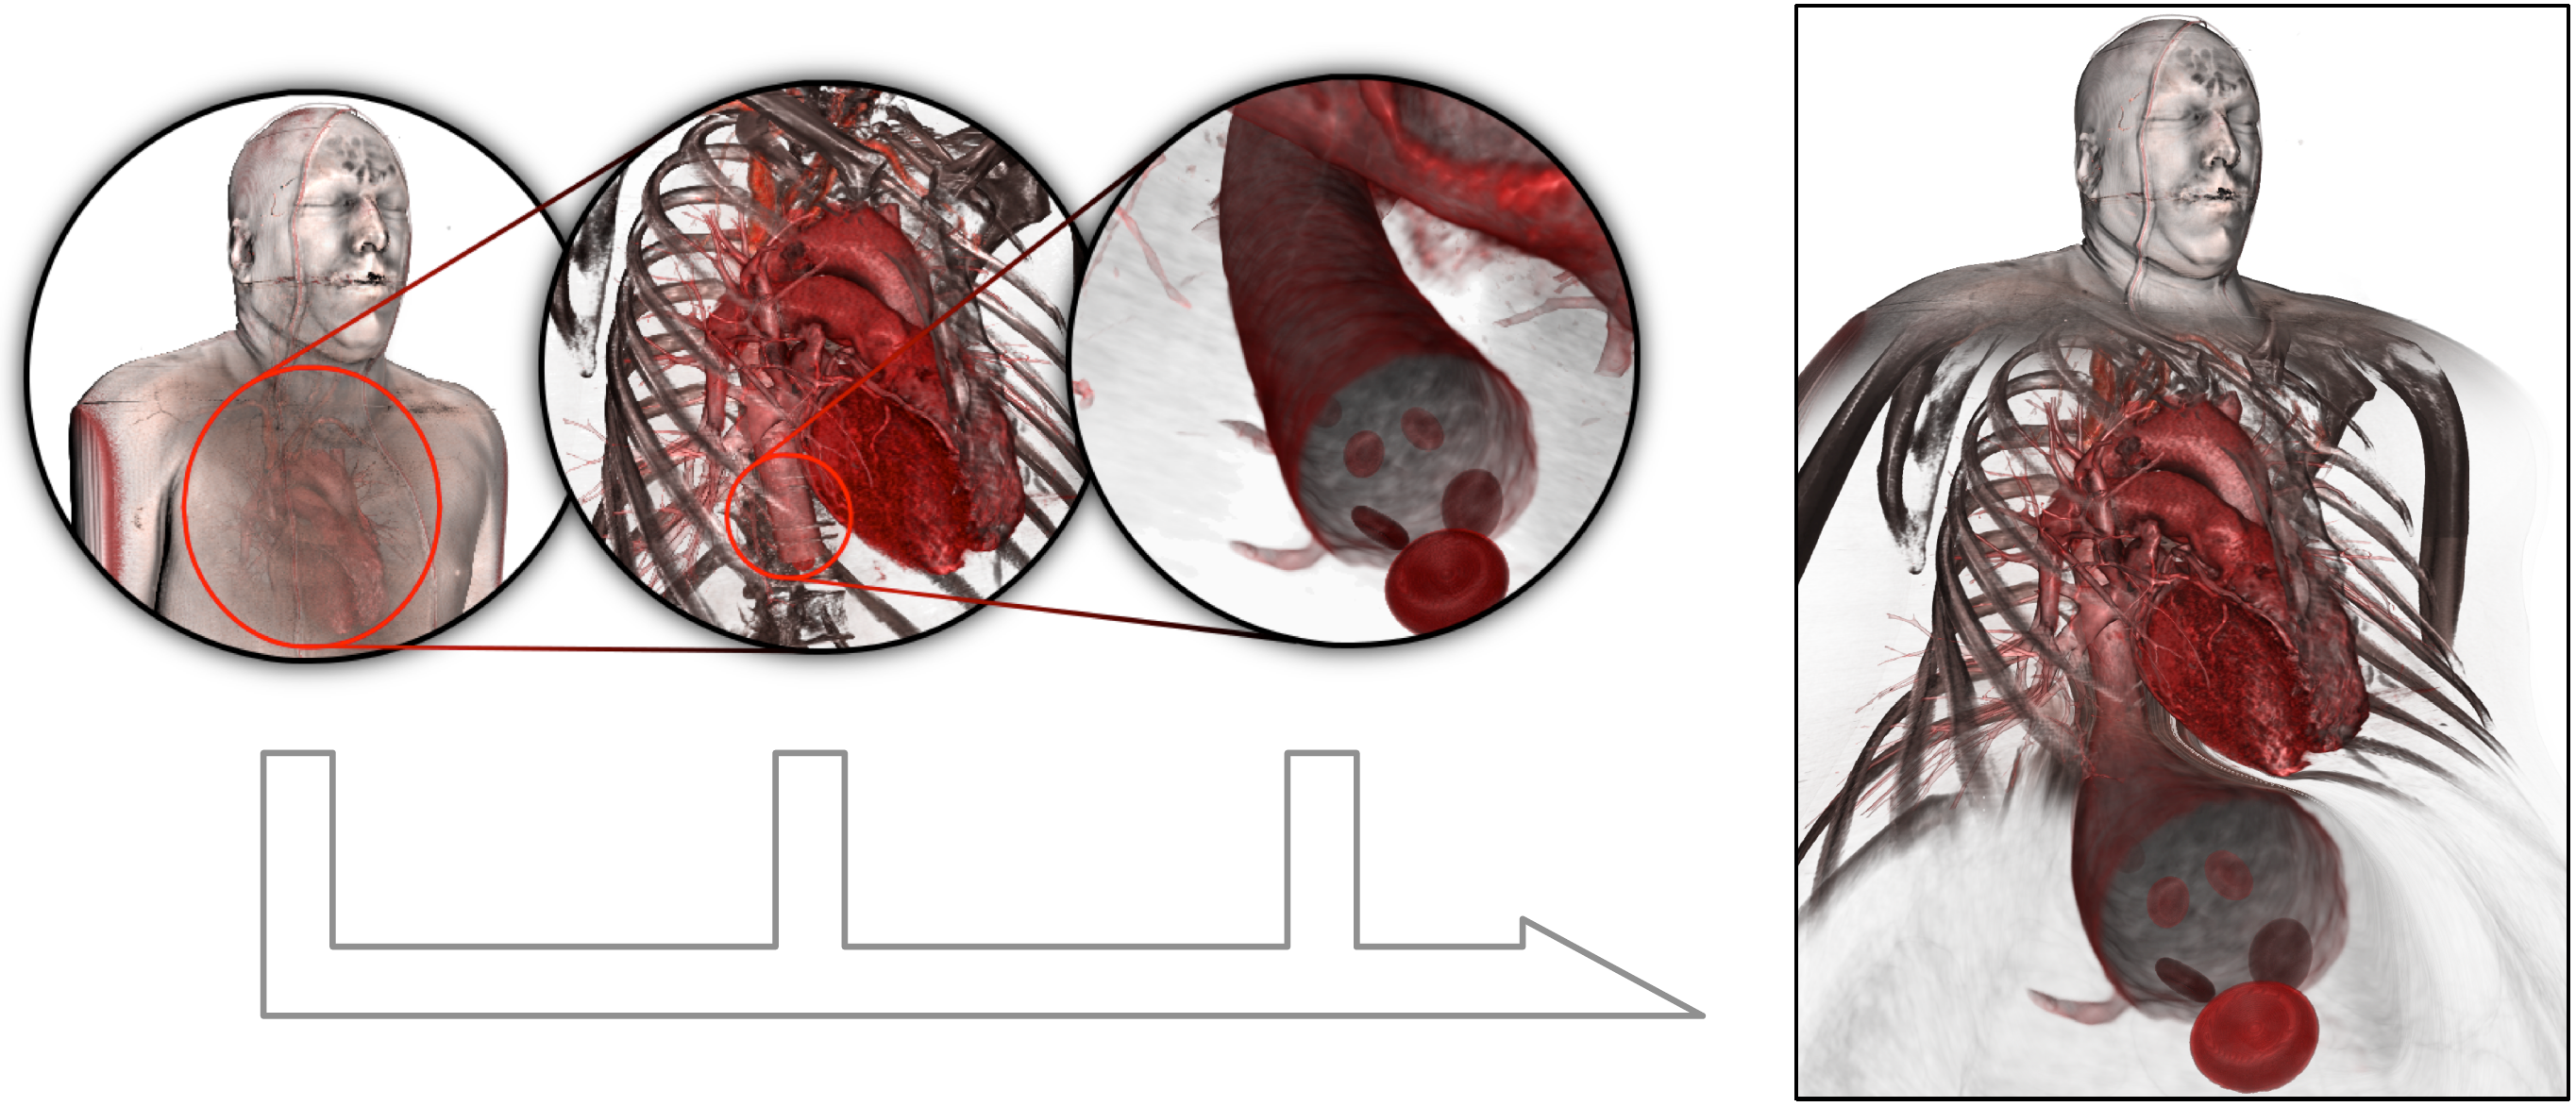
\includegraphics[width=\textwidth]{Figures/multiscale3d}
\decoRule
\caption[ multiscale ]{ A Rendering Framework for Multiscale Views of 3D Models. A continuous multiscale view (right) of a volumetric human body dataset shows three different levels of detail (left three) in a single image. The image on the right is directly rendered with our multiscale framework.}
\label{fig:multiscale}
\end{figure} 
 
  Bruckner and  Groller~\cite{4015467} proposed exploded view for volume data by partitioning the volume into several segments (figure \ref{fig:exploded}). Basically, in an exploded view the object is decomposed into several parts which are displaced so that internal details are visible. This does not only give an unobstructed view on the focus but also potentially reveals other interesting information, such as
cross-sections of the split object. The advantage of exploded views is that they simultaneously convey the global structure of the depicted object, the details of individual components, and the local relationships
among them. A Force-directed layout approach is used to arrange three-dimensional objects
in such a way that they do not occlude another object, but with as little displacement as possible. Four forces are used. \textbf{The Return force } is an attractive force that tries to move the parts towards
their original location. The force $F_r$ is realized as a logarithmic spring:
 \[ F_r=c_{r}\ln(||r||)\cdot \frac{r}{||r||} \] 
 where $r$ is the vector from the vertex's current position to its original location and $c_r$ is a constant factor.
 \textbf{The Explosion force} drives the specified parts away from our selection object. The explosion point is also weighted according to the size of the region corresponding to an octree node. Each explosion point exerts a force $F_e$ on every part $P_i$:
  \[ F_e=  \frac{c_e}{e^{||r||} } \cdot \frac{r}{||r||} \]
  where $r$ is the vector from the explosion point to the closest point of the part geometry of $P_i$ and $c_e$ is a scaling factor.
   \textbf{The Viewing force} is a view-dependent force which attempts to arrange parts so that they do not occlude the selection for the current viewing transformation. The force $F_v$ is:
   \[ F_v=  \frac{c_v}{||r||} \cdot \frac{r}{||r||} \] 
   where $r$ is the vector from the closest point along the viewing ray to the center of the body and $c_v$ is a scaling factor.
   \textbf{The Spacing force} prevents clustering of parts, we also add a
repulsive force $F_s$. For a part $P_i$, the spacing force exerted by another part $P_j$ is:
\[ F_s=  \frac{c_s}{||r||^2} \cdot \frac{r}{||r||} \] 
where $r$ is the vector from the center of $P_j$ to the center of $P_i$ and
$c_s$ is a constant scaling factor. 
\begin{figure}[th]
\centering
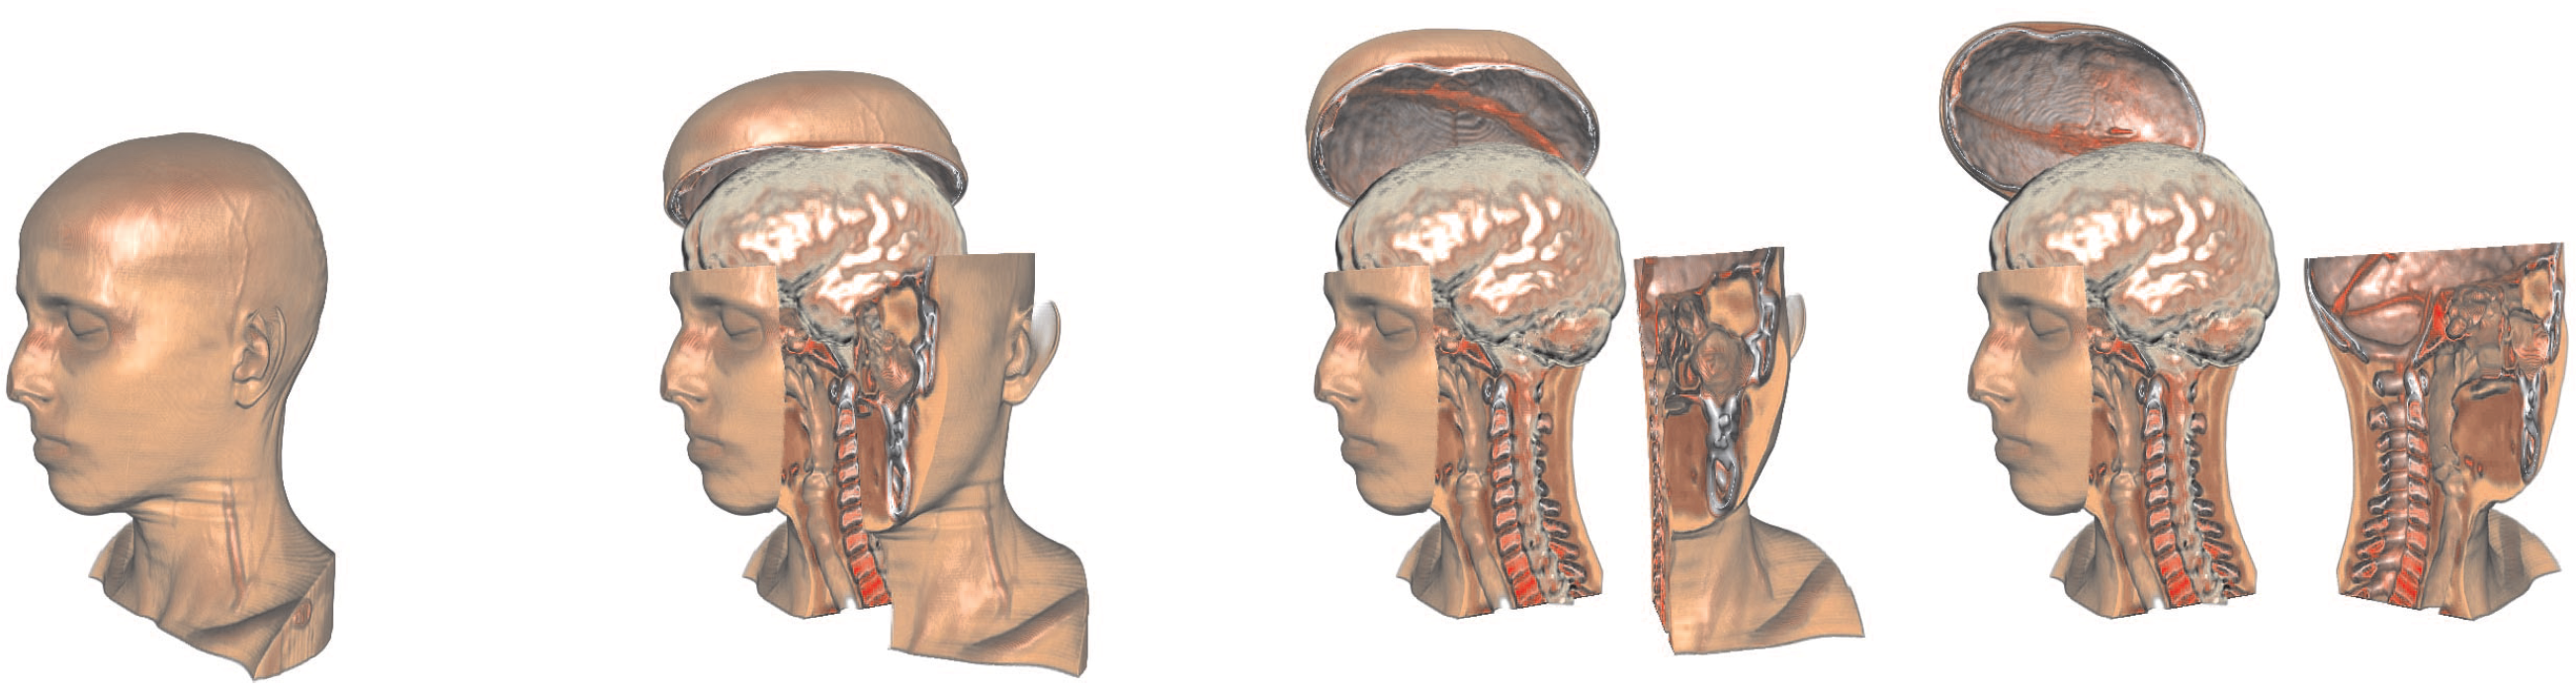
\includegraphics[width=\textwidth]{Figures/explodedview}
\decoRule
\caption[ Interactive exploded-view]{ Interactive exploded-view illustration of a human head with increasing degrees-of-explosion. Two hinge joints are used to constrain part
movement}
\label{fig:exploded}
\end{figure}
  
 
  
  \cite{1250400} performed deformations using peeling to see hidden parts of the data. Their goal in using deformations is to increase the visibility of
the inner portions of the volume, without completely removing the
surrounding data that normally occludes the inside. This is akin to
focus+context schemes that allow a user to zoom-in on data of
interest, while using remaining screen space to show the surrounding
context. Appropriately chosen deformations could, for example,
split open a volume, showing displaced structures side-by-side,
making it easy for the user to see how they connect, and allowing
the user to mentally stitch them together into a whole. Deformations
with familiar real-world analogues (e.g. cutting and peeling
the skin off a fruit, or the layers off an onion) are also likely to be
readily understood by users.
Therefore in their work, they describe a prototype system that implements
different metaphors for deformation-based browsing of volumetric
data. 
As will be seen, a key element of our approach is to support
differential treatment of the various semantic layers in a data set.
The term ''semantic layers'', means subsets of the data that are useful
or meaningful to the user. These layers could be defined geometrically,
for example as sections created with parallel planar cuts.
More typically, layers would depend on the voxel data values, for
example boundaries that are found during segmentation or isosurface
extraction. In the context of medical visualization, there is at
least anecdotal evidence that anatomists, for example, prefer to remove
tissue layer by layer, rather than making
arbitrary planar cuts.
 
 
Deformations can reveal predefined features in the dataset by taking into account the precomputed segmentation. Tong et al. proposed a deforming Lens which moves streamlines to observe the inner part of streamline bundles~\cite{7332955}. 

\begin{figure}[th]
\centering
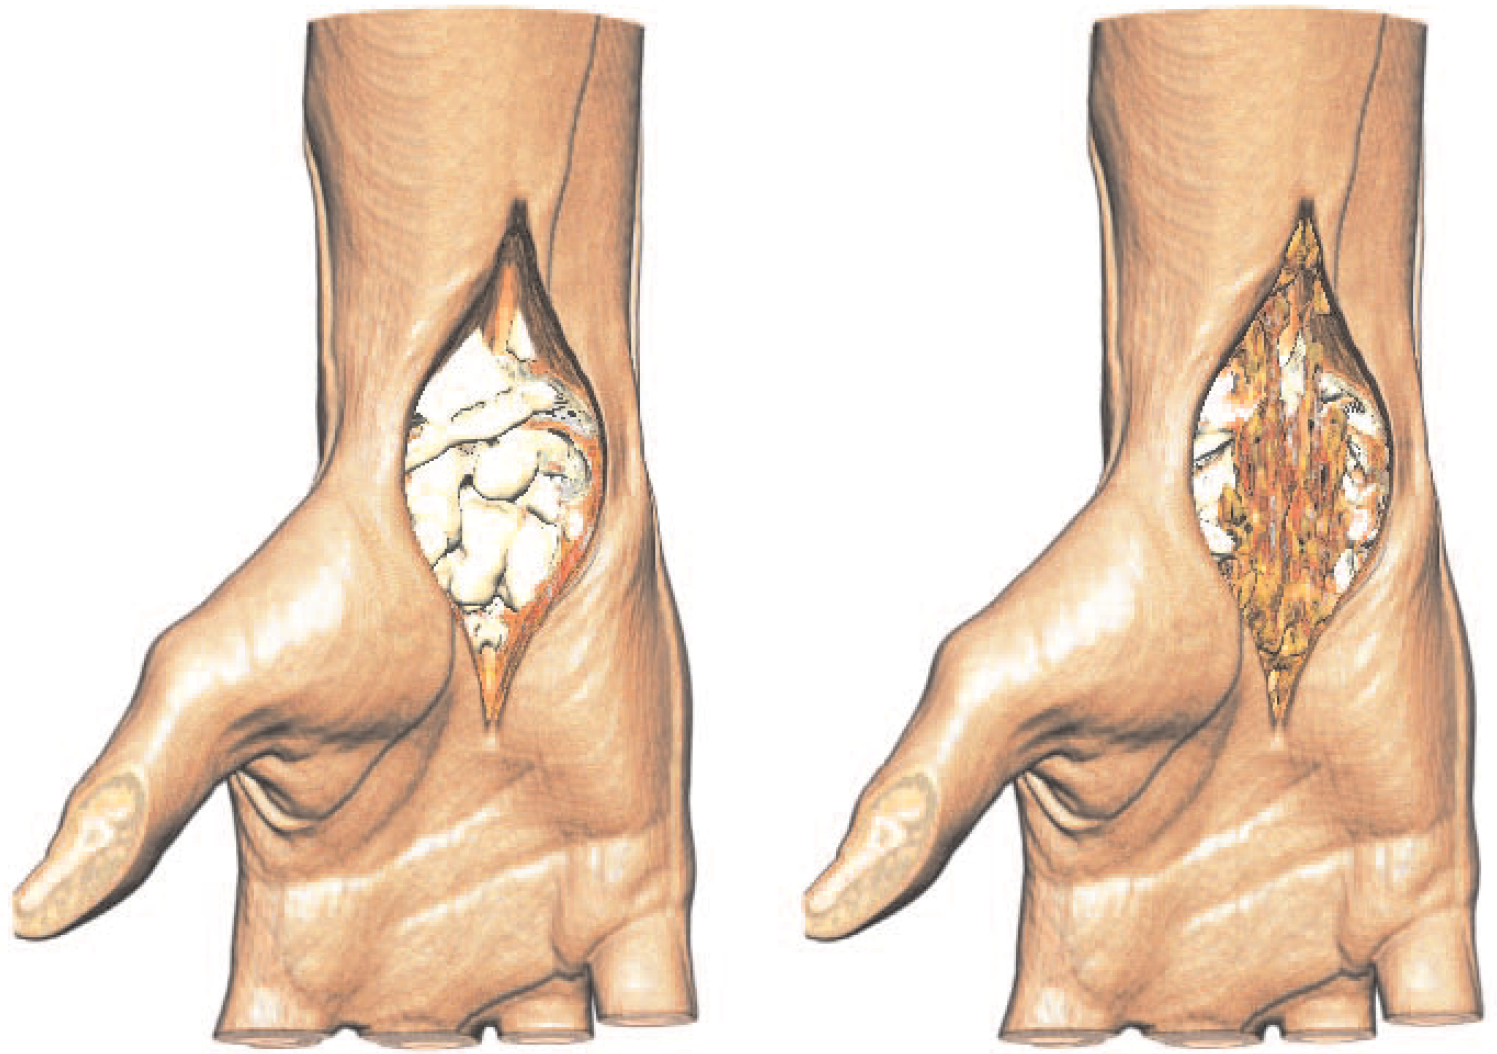
\includegraphics[width=\textwidth]{Figures/cut}
\decoRule
\caption[ Feature Aligned Volume Manipulation]{ A feature-aligned retraction applied to a human hand data set, showing bones (left) and vessels (right)}
\label{fig:cut}
\end{figure}
\cite{Correa:2007:IDD:1313046.1313163} proposed a framework  allowing the users to physically or actively manipulate the geometry of a data object. Some studies performed deformations using surgical metaphors like ~\cite{4069230,Correa:2006:FAV:1187627.1187827} to see hidden parts of the volume, see figure \ref{fig:cut}. They propose a feature-based technique for manipulating volumetric objects for illustrative visualization, and describe a GPU-based implementation that enables interactive specification and their rendering.
Inspired by medical illustrations that frequently
depict the results of manipulation with tools such as peelers,
retractors and pliers, this system allows the specification of manipulation
through a collection of procedurally-defined manipulation operators.



\begin{figure}[th]
\centering
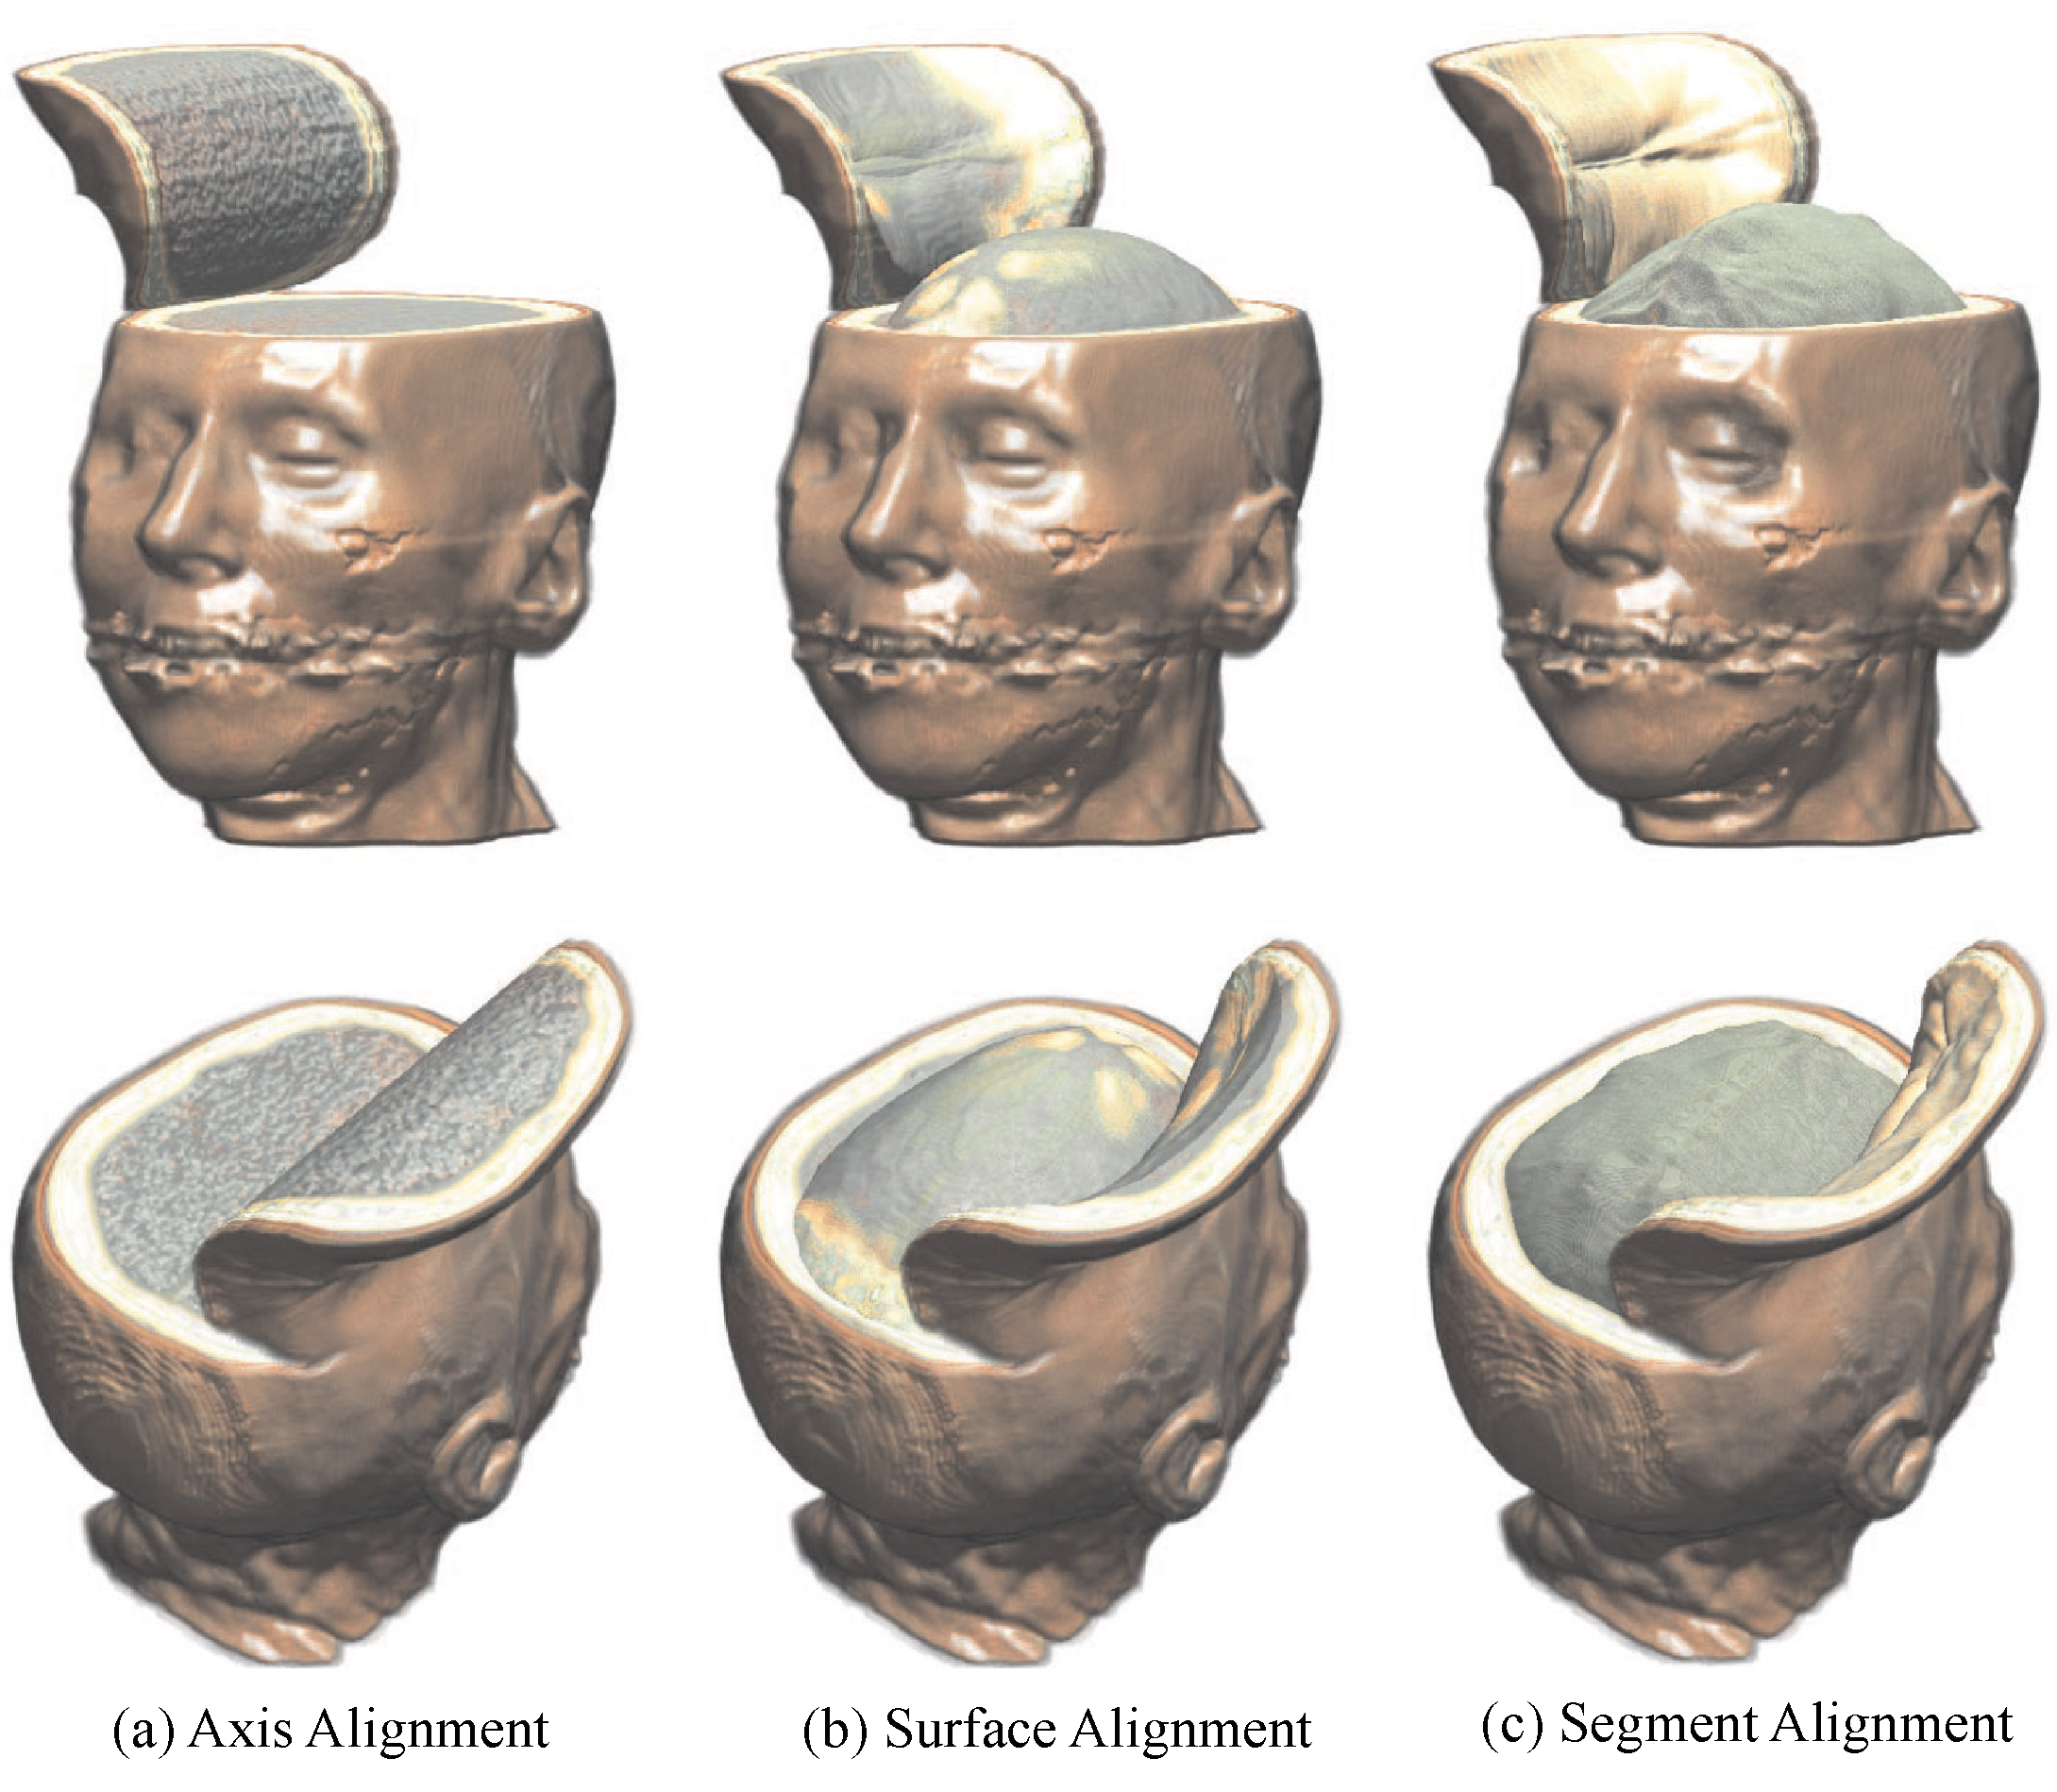
\includegraphics[width=\textwidth]{Figures/peel.pdf}
\decoRule
\caption[ Feature Aligned Volume Manipulation]{ An example of different types of alignment. (a) Axis aligned peel. Note how the peeled layer is thick and flat, since it is aligned with
an orthogonal axis. (b) Surface aligned peel, aligned with a computed
distance field. Notice how it approximates a surface. (c) Segment
aligned peel, based on segmentation, which is more accurate. Note
that in the feature based alignment (b) and (c) the peel is thin and
rounded.}
\label{fig:peel}
\end{figure}

 Correa et al. introduced two feature-based methods, namely surface alignment and segment alignment for modeling and rendering illustrative manipulation, and compare them with the traditional axis alignment method, see figure \ref{fig:peel}. They devise a method for estimating accurate normals along the surface of cuts
and dissections while maintaining continuous normals, which allows
us to obtain correct shading of the object being manipulated, opaque
or translucent. The four operators proposed in this framework are the following:
\begin{itemize}
\item Peeler: The peeler simulates peeling or cutting of the outer layers
of a volumetric model. Different parameters
of the peeler, such as thickness of the cut and the angle of bending of
the peeled layer, can be manipulated interactively to obtain different
illustrative effects.
\item Retractors: In the context of surgical illustration, retractors are tools used to spread organs or bones, or to hold back soft tissues such as
skin. In the context of illustration, they are useful for illustrating the
access to the internal organs.
\item Pliers: Pliers are tools used to grasp tissue and pull it or poke it into the volumetric object. The operator parameters include the shape of
the displacement and the radius of influence which specifies how the
displacement propagates through the volume.
\item Dilator: Dilators are used to gain access into narrow regions, cuts
or vessels. They essentially scale the region from the inside typically
by blowing air, to increase the visibility or accessibility of the region.
When applied to volumetric manipulation, dilators have a similar effect
to that of volumetric magic lenses (\cite{1532818}).
\end{itemize} 
However this framework do not offer tools for local manipulation and exploration inside the cut, which allows perceiving a target under a different perspective while keeping the global context. 


\cite{6787171} propose a set of linked views that display
subsets of data attributes. Example views are 3D DVR plots, 2D
scatterplots, and 2D and 3D histograms. Views are linked by brushing
and free-form selection. Using the optimal view(s), one can find structures
of interest, e.g. spatially compact zones in DVR renderings or peaks in histograms, and highlight or erase such structures in all views
at once. They enhance classical histogram views with shading, sorting,
and depth, to allow spotting complex patterns with greater ease. In addition, they
propose a smooth animation between multiple views, to locate (and select)
data patterns which are hard to isolate in static plots. This framework integrate
a Focus+Context deformation that adds the ability to uncover locally occluded
spatial patterns in different views. The GPU implementation of their
techniques, which they call color tunneling, creates real-time interactive,
animated, explorations of datasets of tens of millions of points
on a modern PC. Since the goal is to explore dense multivariate datasets which exhibit significant
overlap between groups of voxels or pixels, tools to
interactively unveil the occluded structures of interest are needed.
Five interactive techniques have been proposed as follows (see figure \ref{fig:colortunneling}):
\begin{itemize}
\item View linking: Three configurable views (2 exploration views and
one lock view) for data exploration,
\item Warp: Animates a view between two configurations,
\item Lock: Locks items not to be affected by brush or dig ,
\item Brush: With the lock view, brushing allows adding or removing
data in a view,
\item Dig: With the lock view, digging pushes data points away from
the lens center to unveil occluded structures 

\end{itemize}

\begin{figure}[th]
\centering
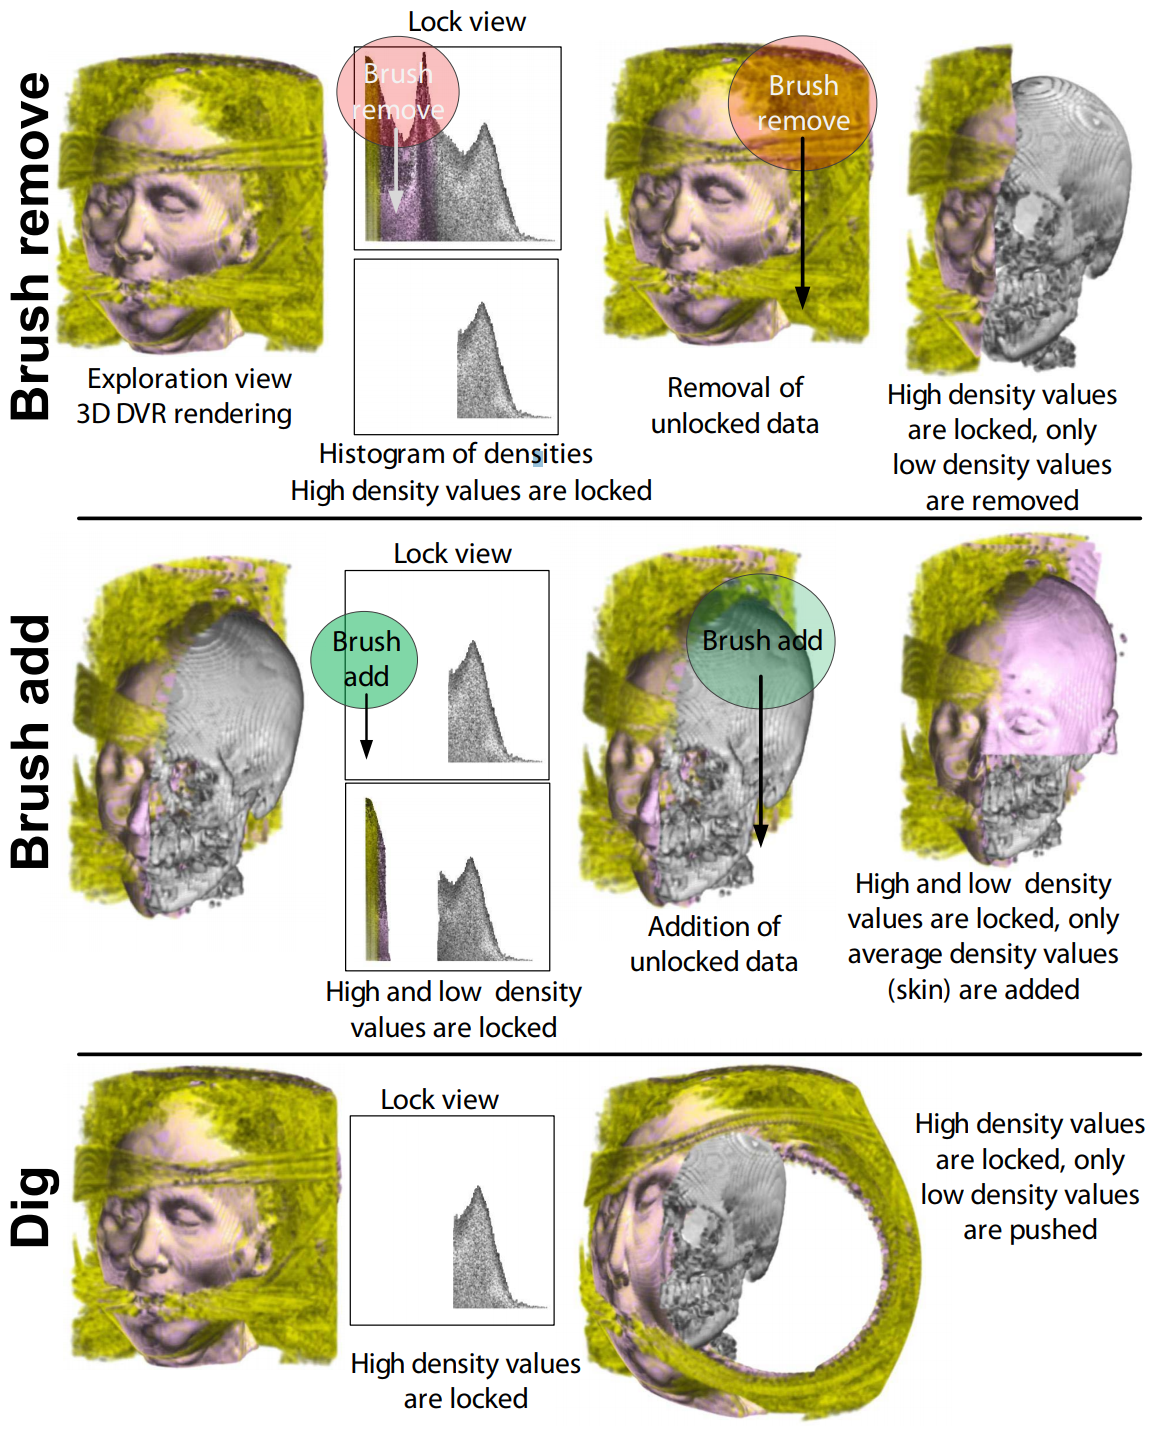
\includegraphics[width=\textwidth]{Figures/colortunneling}
\decoRule
\caption[ Color Tunneling]{ Brush, dig, and lock tools. Locked items are not affected by
brush and dig. We used transfer functions to make air voxels transparent
and standard gradient shading. We see that the head is surrounded by a
large amount of uninteresting noise (yellow).}
\label{fig:colortunneling}
\end{figure}


\section{Volume rendering in Virtual Reality and Augmented Reality}

\subsection{ Remote volume rendering}

Volumetric data exploration with direct volume rendering technique is of great help to visually extract relevant structures in many fields of science: medical imaging ~\cite{ljung_full_2006}, astrophysics and more recently in baggage inspection. To leverage this knowledge extraction, many techniques have been developed. 

In this section, we detail existing ones with volume visualization, transfer function, direct voxel manipulation, and focus plus context interaction.
Volume visualization can be done with geometric rendering system which transforms the data into a set of polygons representing an iso-surface. The contour tree algorithm ~\cite{carr_computing_2000} and other alternatives such as branch decomposition ~\cite{pascucci_multi-resolution_2004} are usually used to find these iso-surfaces. According to H. Guo ~\cite{guo_local_2013}, contour trees algorithms are vulnerable to noises, which can be problematic in baggage inspections since dense materials (e.g. iron) cause noises by reflecting the X-rays. For this reason we used the volume rendering technique; Chen et al. provide a review of existing techniques ~\cite{chen_3-d_2000}.
In order to investigate volumetric dataset, one can use the Transfer Function (TF). In practice, it maps the voxel density with a specific color (including its transparency). Transfer function can be 1D, 2D or nD and are of great help to isolate structures of interest in volumetric data ~\cite{kniss_multidimensional_2002}. Thanks to the color blending process, suitable transfer function can also reveal iso surface or hide density to improve the volumetric data visualization. The setup of this transfer function remains complex, but some automatic systems provide solution thanks to data analysis ~\cite{correa_size-based_2008} ~\cite{sereda_visualization_2006} ~\cite{patel_moment_2009} or user interactions ~\cite{guo_wysiwyg_2011}. Since our users have a limited knowledge on volume rendering, we developed new interaction techniques with sufficient abstraction level regarding technical constraints. These techniques will be detailed in this paper. As an example, we investigated predefined transfer functions with smooth transitions when changing their setup to reduce disruptive animation effects ~\cite{tversky_animation:_2002}.
Since graphic card power never stops to improve, new techniques allow the direct manipulation of the voxels which composes the volume to be displayed. Color tunneling introduced a set of interactions (lock, Brush, Dig) to explore 2D and 3D dataset composed of pixels of voxels ~\cite{hurter_interactive_2014} with point based rendering techniques ~\cite{sainz_point-based_2004} . Histomage also provides direct manipulation of pixels thanks to a histogram which can be used as a new selection and pixel modification tool ~\cite{chevalier_histomages:_2012}. Other interactive systems investigated pixel exploration with a lens as a focus plus context technique ~\cite{elmqvist_color_2011} ~\cite{hurter_moleview:_2011}. Our work provides additional interaction techniques with pixel based techniques ~\cite{hurter_interactive_2014} to address occlusion issues, focus and context awareness, reversibility of the actions, and continuity.  